\documentclass[fleqn]{article}

\makeatletter
\newcommand{\vo}{\vec{o}\@ifnextchar{^}{\,}{}}
\makeatother
\usepackage[utf8]{inputenc}
\usepackage{amsmath}
\usepackage{amssymb}
\usepackage{graphicx}
\usepackage{hyperref}
\usepackage[section]{placeins}

\title{COMS3007A\\Machine Learning\\Assignment}
\author{Mpendulo Nxumalo\\ 2154519\\ \\Vusumzi Booi\\2109688}
\date{May-June 2021}

\begin{document}
	\maketitle
	\newpage
	
	\section*{Description of Dataset}
	
		\subsection*{Source of dataset}
			
			the dataset was retrieved from the following link: \\
			\url{https://www.kaggle.com/arashnic/covid19-hospital-treatment}\\
			\\The data was collected from multiple hospitals during the breakout of 	the Covid-19 pandemic (march 2020) till recently (May2021).The data was collected 	so that predictions may be made to determine how long an individual may spend in hospital if they are hospitalised due to Covid-19. This information will be used by hospitals for optimal resource allocation and better functioning.
			
			
			
		\subsection*{Summary of the Dataset}
			 The dataset consists of 318438 records and 18 features. \\
			 \\ the features being \\
			 \begin{itemize}
			 	\item case id 
			 	\item Hospital
			 	\item Hospital type
			 	\item Hospital city
			 	\item Hospital region
			 	\item Available Extra Rooms in Hospital
			 	\item Department
			 	\item Ward Facility
			 	\item Bed Grade
			 	\item patient id
			 	\item City Code Patient
			 	\item Type of Admission
			 	\item Illness Severity
			 	\item Patient Visitors
			 	\item Age
			 	\item Admission Deposit
			 	\item Stay Days
			 \end{itemize} 		 
			The target in this dataset will be Stay Days. The patient id and case id will not be used in the analysis and predictions made on the dataset, as it does not have much significance 
			
		\subsection*{Target: Stay Days}
			
			The target Stay Days consists of the following possible values:\\
			
			\begin{itemize}
				\item 0-10
				\item 11-20
				\item 21-30
				\item 31-40 
				\item 41-50
				\item 51-60
				\item 61-70
				\item 71-80
				\item 81-90
				\item 91-100
				\item More than 100 Days   
			\end{itemize}
			
			where each target represents a time frame in which a patient hospitalised will recover. Death is not included as the data was collect on individuals 					who were hospitalised and survived covid 19.\\
			\\plotting the data we obtain Figure~\ref{fig:1} and Figure~\ref{fig:2}\\			
			\begin{figure}[hb]
  				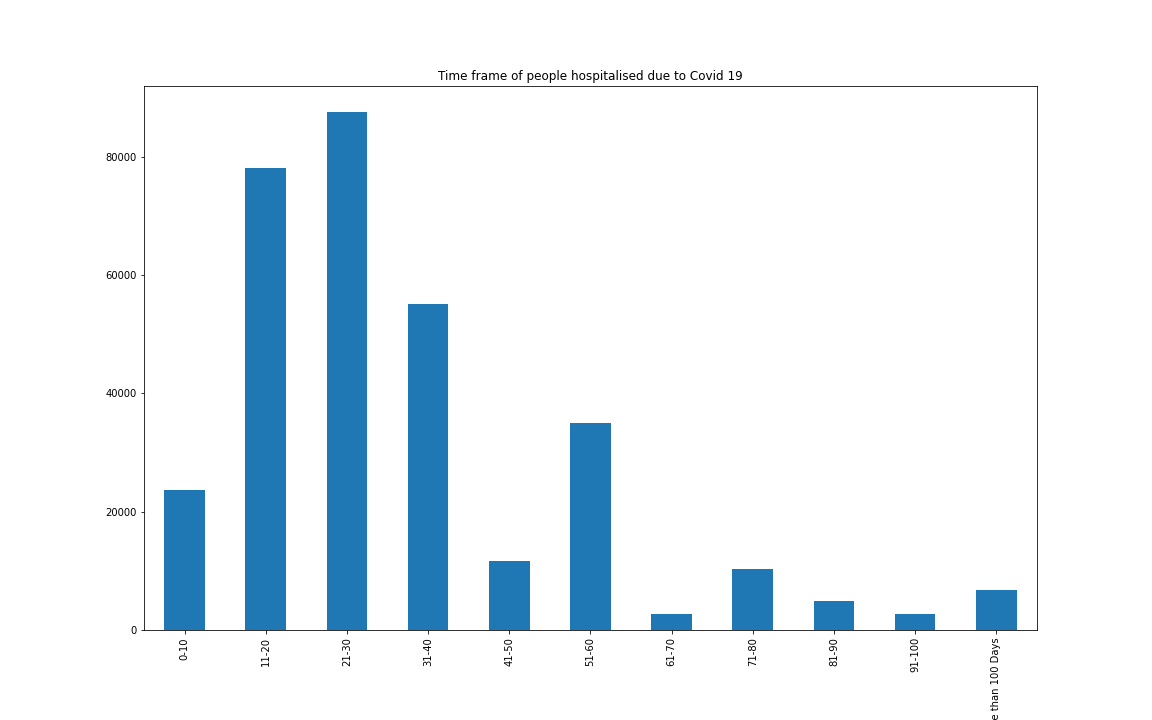
\includegraphics[width=\linewidth]{clas_hist.png}
  				\caption{Histogram of the number of people that stayed in each time 						frame}
  			\label{fig:1}
			\end{figure}
			\FloatBarrier
			\begin{figure}[hb]
  				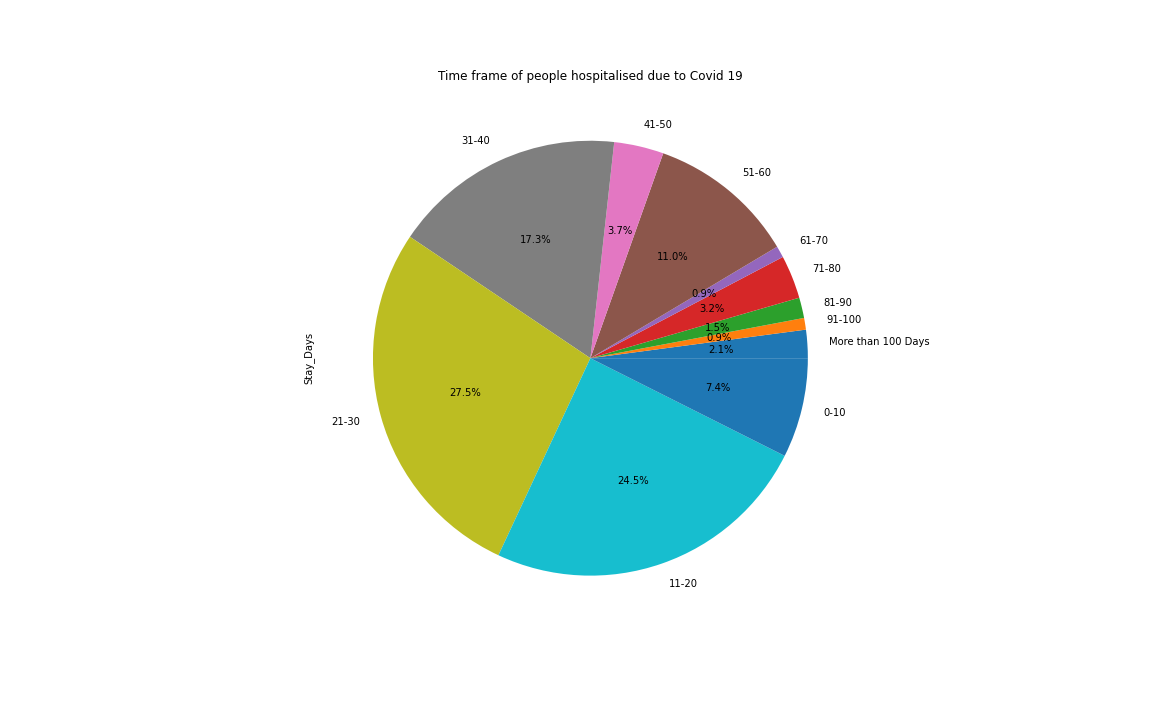
\includegraphics[width=\linewidth]{class_pie.png}
  				\caption{Pie chart of the number of people that stayed in each time 						frame}
  				\label{fig:2}
			\end{figure} 
			\FloatBarrier
			
			After analysing the charts the following insights may be concluded: \\
			Most people infected with Covid-19  recover within 0-30 days of contracting the virus.
			This observation agrees with the medical experts opinion on the recovery time frame 			of Covid 19.
			
		\newpage
		\subsection*{Hospital}
			This feature gives information on which hospital the person was treated.
			Plotting the results we obtain \\ 
			\begin{figure}[hb]
  				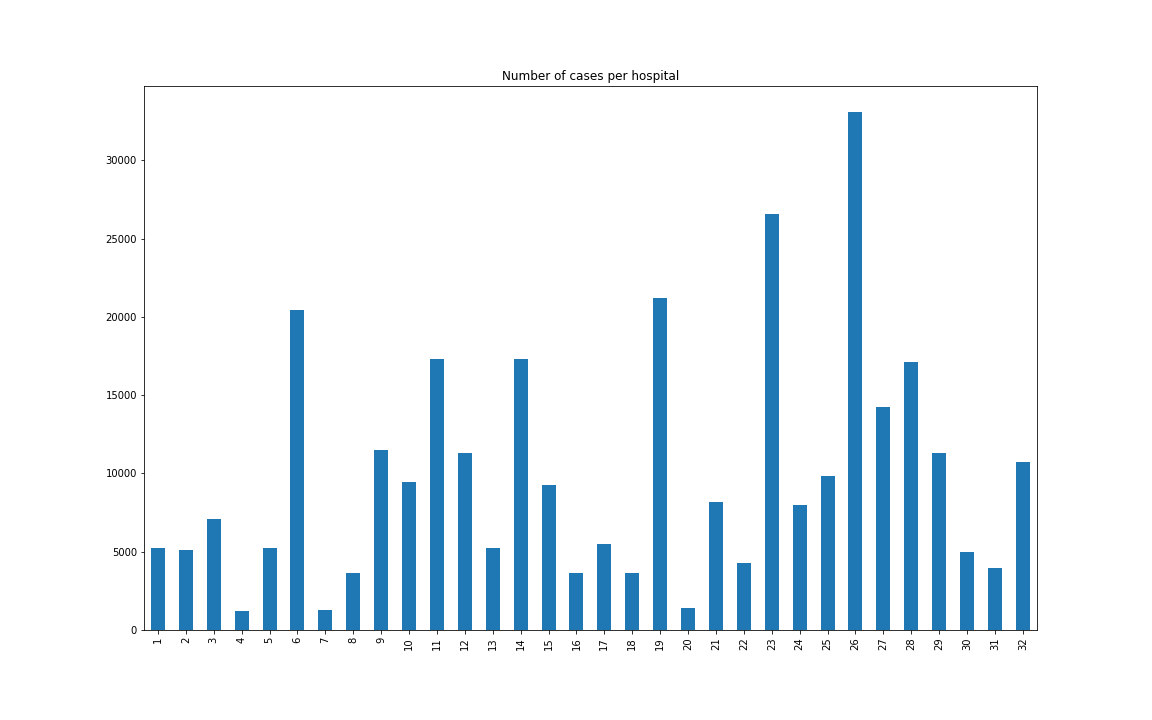
\includegraphics[width=\linewidth]{hospital_hist.png}
  				\caption{histogram showing how many cases were handled in each 							hospital}
  				\label{fig:3}
			\end{figure} 
			\FloatBarrier
			From this figure we can see that majority of the cases were handled by Hospital 26. This may be due to numerous factors, to list them they could be due to the population density near the hospital and the cost of services.
		
		\newpage
		\subsubsection*{Hospital Type}
			This feature gives a description of the type of hospital that treated the case. When plotting this data we obtain the following figure: \\
			\begin{figure}[hb]
  				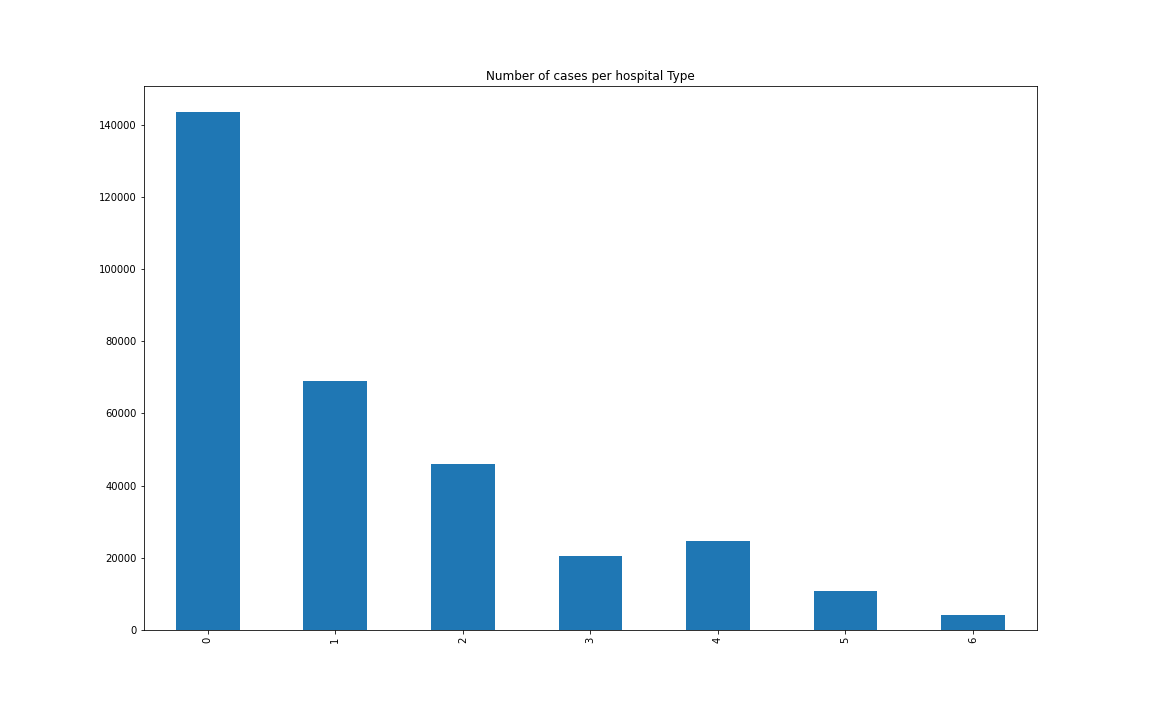
\includegraphics[width=\linewidth]{hospitalType_hist.png}
  				\caption{histogram showing how many cases were handled in each type of hospital}
  				\label{fig:4}
			\end{figure} 
			\FloatBarrier
			
			From the figure we can deduce that hospital type 0 handled majority of the cases.This could imply that hospital 0 is the most effective hospital type in handling Covid-19 cases.
		\newpage
			
		\subsection*{Hospital City}
		This feature indicates the number of people hospitalized due to the Covid-19 virus in the respective cities
		
		    \begin{figure}[hb]
  				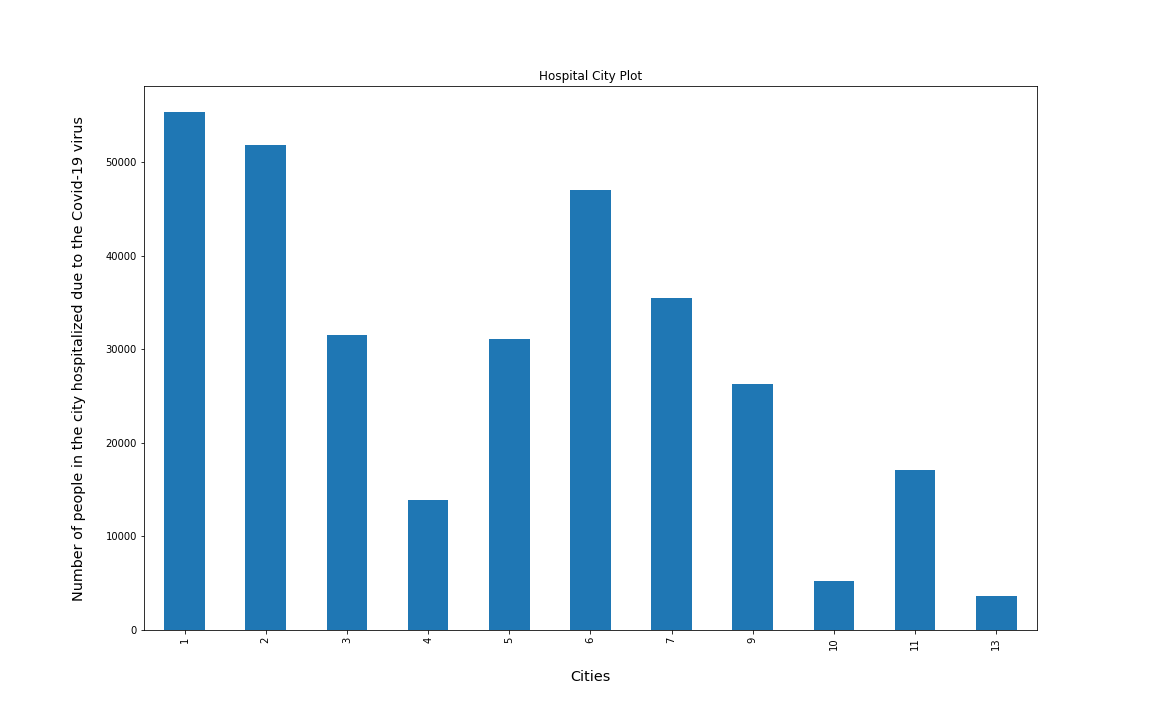
\includegraphics[width=\linewidth]{hospitalCity_hist.png}
  				\caption{histogram showing the number of people hospitalized due to the Covid-19 virus in the respective cities}
  				\label{fig:5}
			\end{figure} 
			\FloatBarrier
			
			From the figure we can deduce that the city 1 is the city with the most people hospitalized due to the Covid-19 virus, which is followed closely by city 2 and city 6 respectively.This can imply that city 1, city 2 and city 6 are Covid-19 virus hotspots.
			
			
		\newpage	
		\subsection*{Hospital region}
		This feature indicates the number of people hospitalized due to Covid-19 virus in a particular region
		
		
		    \begin{figure}[hb]
  				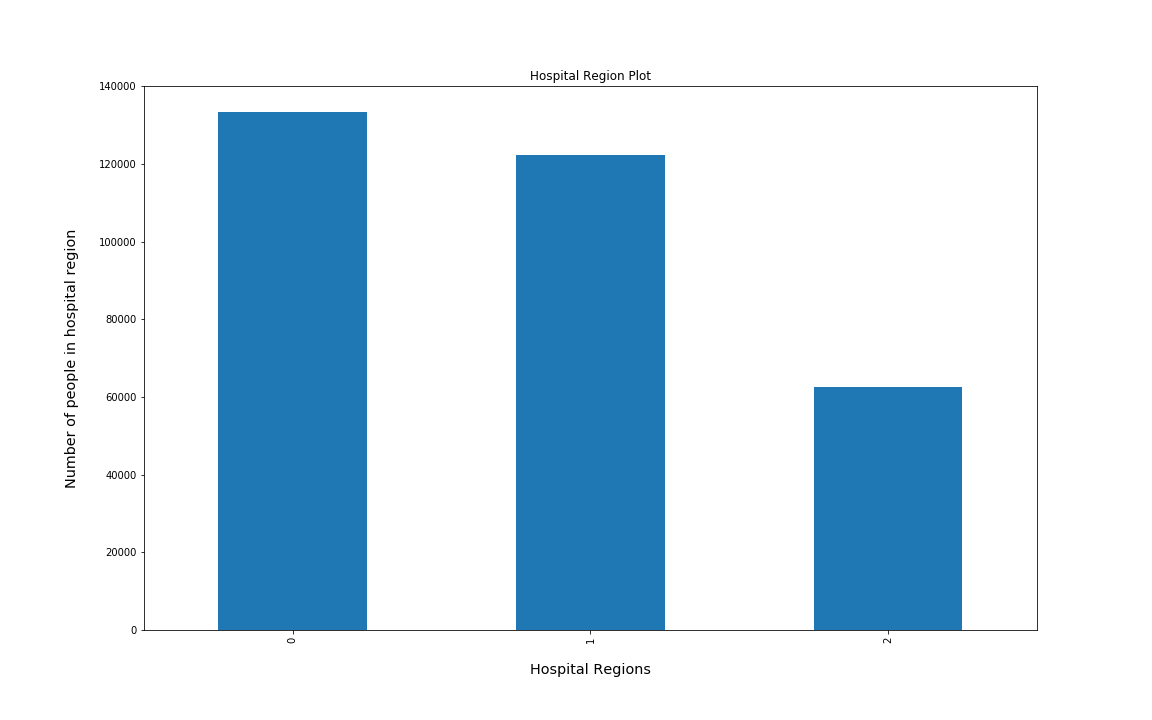
\includegraphics[width=\linewidth]{hospitalRegion_hist.png}
  				\caption{histogram showing the number of people hospitalized due to the Covid-19 virus in the respective cities}
  				\label{fig:6}
			\end{figure} 
			\FloatBarrier
			
			
		From the figure above we can deduce that region 1 has the most people hospitalized due to covid-19 virus followed by region 2 and region 3 respectively.
		
		\newpage
		
		\subsection*{Available Extra Rooms in Hospital}
			This feature gives an indication on how many extra rooms the hospital where the patient was admitted has. When plotting the data we obtain the following graph:
			
			\begin{figure}[hb]
  				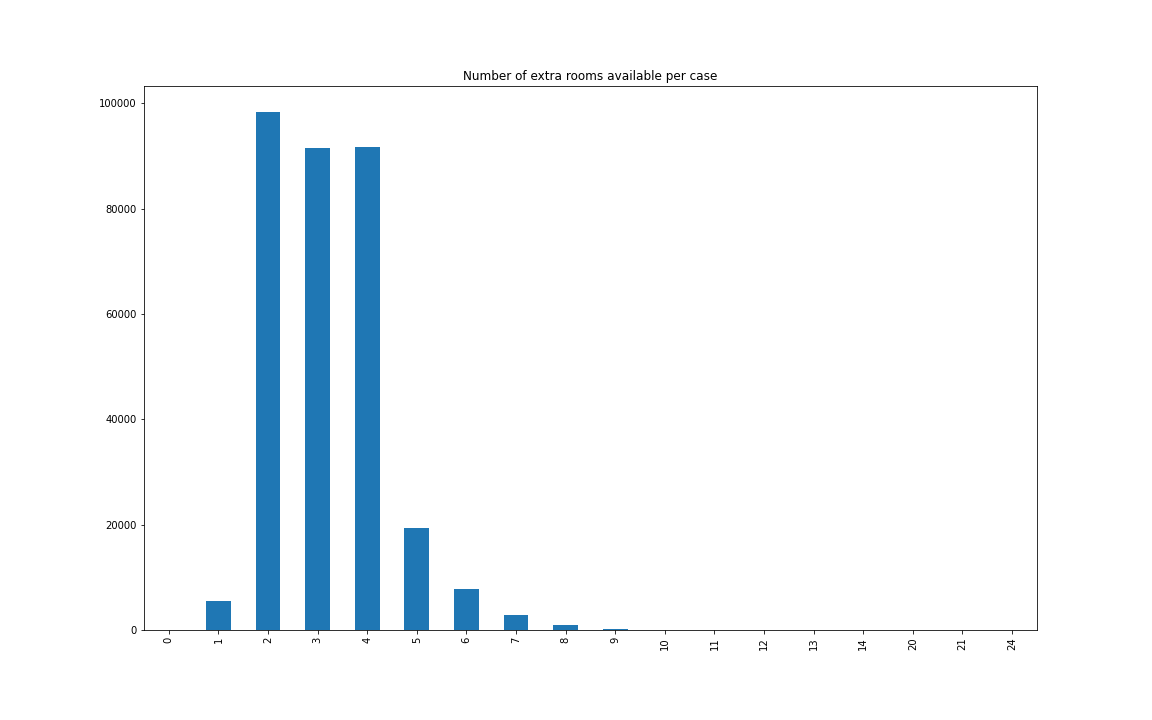
\includegraphics[width=\linewidth]{Extraroom_hist.png}
  				\caption{histogram showing how many rooms where available at time 						patient admitted}
  				\label{fig:7}
			\end{figure} 
			\FloatBarrier
			
			From analysing the figure we may conclude that when a person was admitted to the hospital there was on average between 2-4 extra rooms available
			
		\newpage
		\subsection*{Department}
			This feature gives an indication in which department handled the case in the hospital. Plotting this data we obtain the following figure:
			
			\begin{figure}[hb]
  				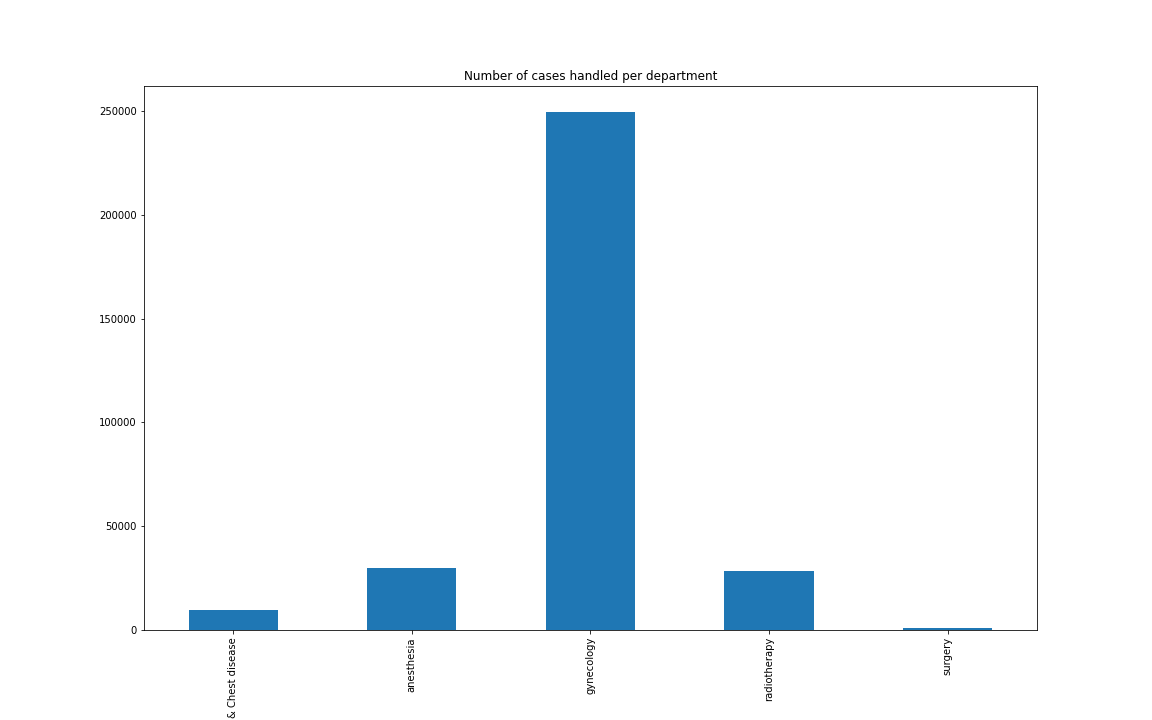
\includegraphics[width=\linewidth]{department_hist.png}
  				\caption{number of cases handled by each department}
  				\label{fig:8}
			\end{figure} 
			\FloatBarrier
			
			As seen in the figure above the department of gynecology handled an extremely large proportion of the cases. This may be due to the availabilty of the staff assigned to that department, covid-19 virus cases were spiking so getting any medical help would of made sense
			
		\newpage
		\subsubsection*{Ward Facility}
		 This feature gives an indication on how many cases were treated in each ward type plotting the data we obtain the following figure:
		 
		 \begin{figure}[hb]
  				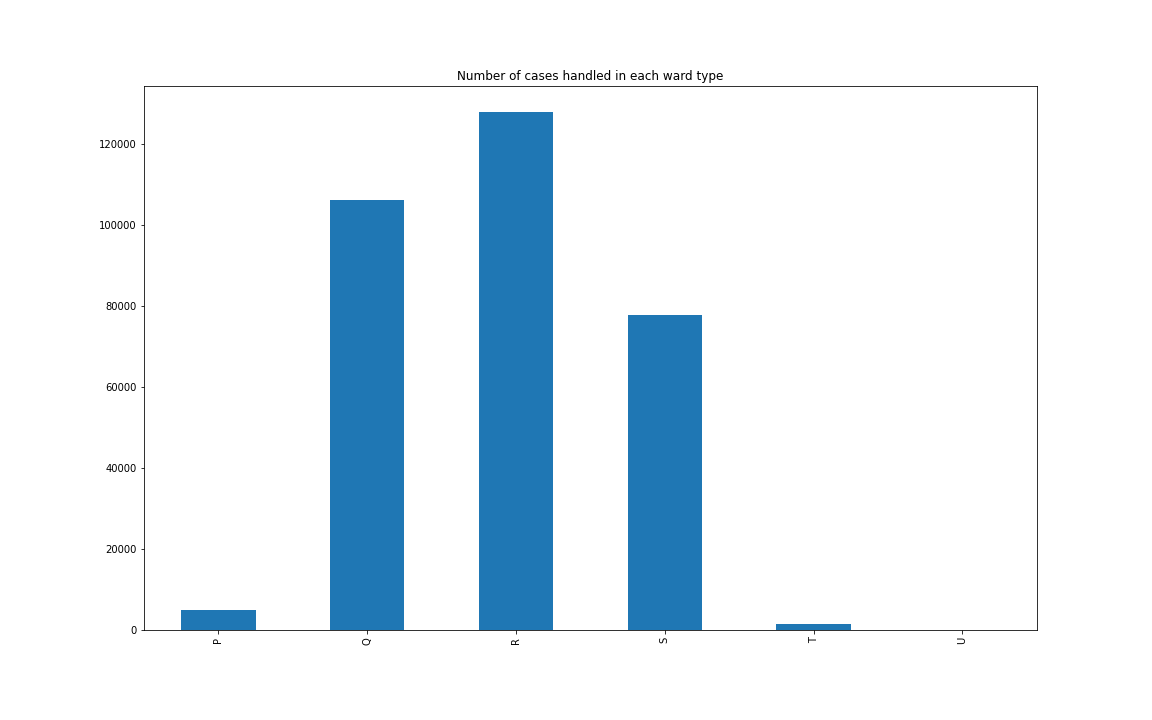
\includegraphics[width=\linewidth]{ward_hist.png}
  				\caption{number of cases handled by each ward type}
  				\label{fig:9}
			\end{figure} 
			\FloatBarrier
			
		As seen in the figure above ward type R handled majority of the cases. This 			may be due to the resources allocated to that ward type such as stuff, 					medicine etc
		
		\newpage
		\subsection*{Bed Grade}
			This feature gives us an indication on the quality of the beds used and the quantity of each type that was used. Plotting this data we obtain the following figure:	
			
			 \begin{figure}[hb]
  				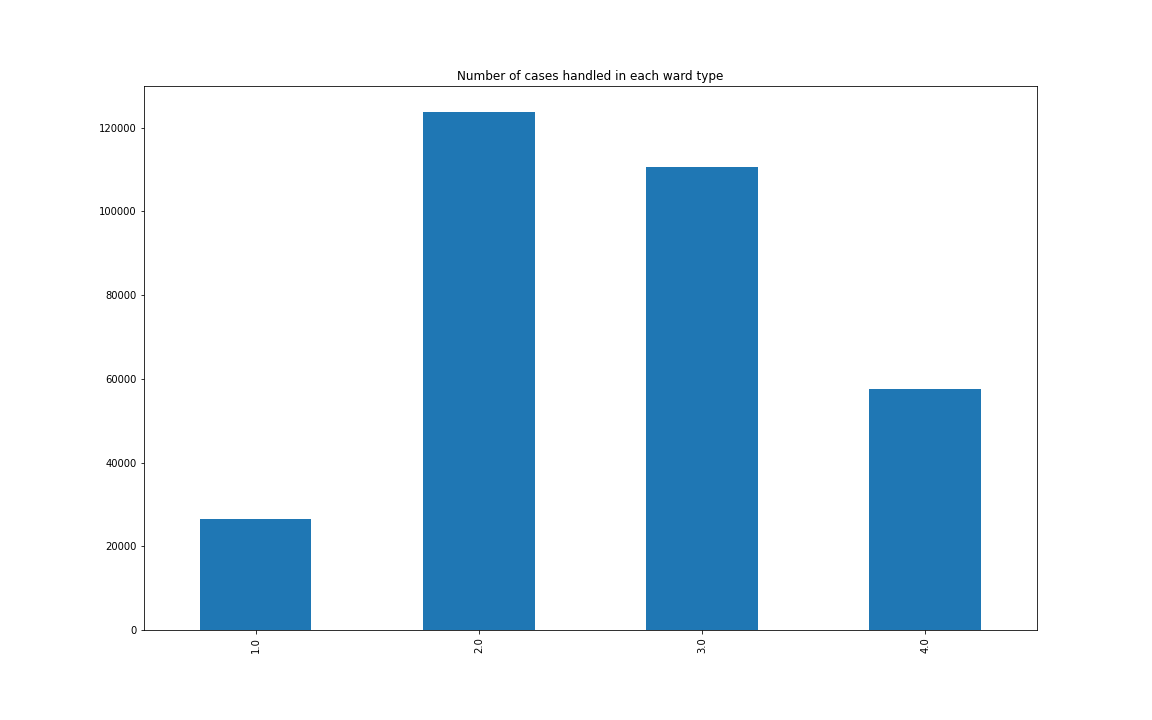
\includegraphics[width=\linewidth]{bed_hist.png}
  				\caption{number of beds assigned to patients of each grade}
  				\label{fig:10}
			\end{figure} 
			\FloatBarrier	
			
			From the figure above its clear that average beds were used majority of the time. This my be due to the financial strain brought by covid 19.
			
		\newpage
		\subsection*{Type of Admission}
			This feature describes the sense of urgency required for this case. Plotting the data we obtain the following figure:
			
			\begin{figure}[hb]
  				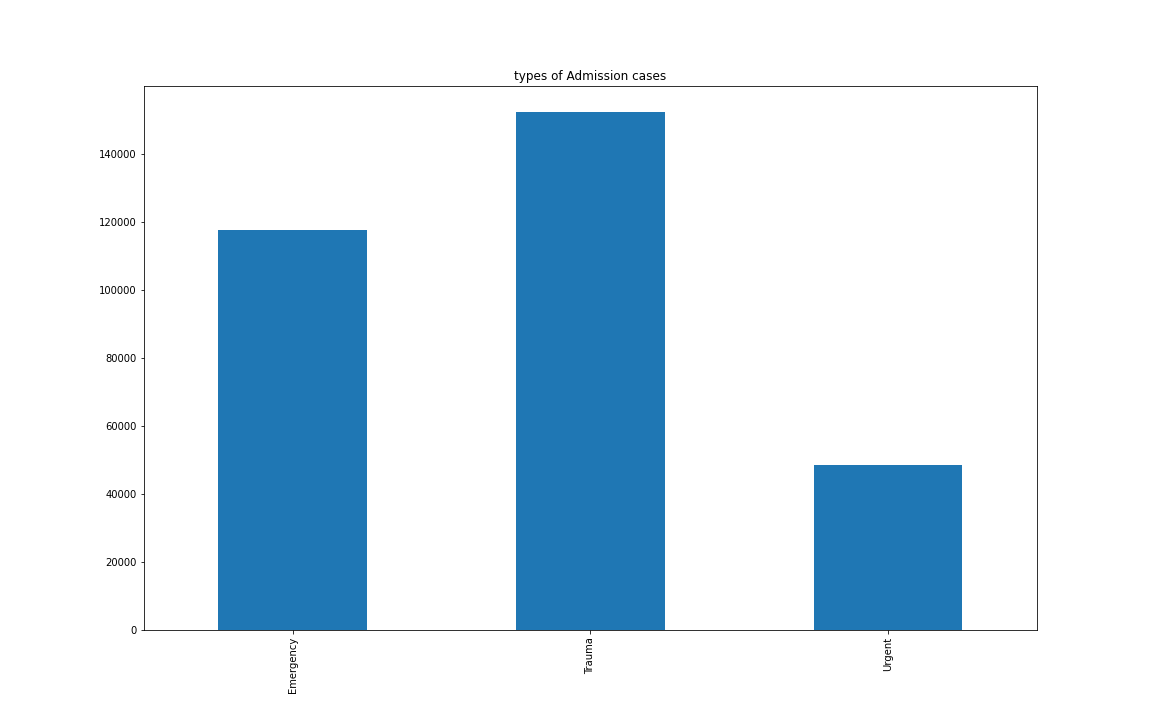
\includegraphics[width=\linewidth]{admin_hist.png}
  				\caption{types of Admission cases}
  				\label{fig:11}
			\end{figure} 
			\FloatBarrier
			
			As seen from the figure above majority of cases were considered trauma cases. This makes sense as for someone to be admitted to hospital due to covid-19 the patient is probably experiencing server symptoms.
			
		\newpage
	\section*{Data Processing}
	The data was processed as follows:
	\begin{enumerate}
        \item We removed the case id, patient id and admission deposit as it did not carry any significance in creating the models to be used
        \item We encoded the entries for the Department feature as follows:
            \begin{center}
            \begin{tabular}{ |c|c| } 
             \hline
             feature value & Encoding\\
             \hline
             gynecology & 0 \\ 
             anesthesia & 1\\ 
             radiotherapy & 2\\
             TB/Chest disease & 3\\
             surgery & 4\\
             \hline
            \end{tabular}
            \end{center}
        \item We encoded the entries for the Ward type feature as follows:
            \begin{center}
            \begin{tabular}{ |c|c| } 
             \hline
             feature value & Encoding\\
             \hline
             P & 0 \\ 
             Q & 1\\ 
             R & 2\\
             S & 3\\
             T & 4\\
             U & 5\\
             \hline
            \end{tabular}
            \end{center}
        \item We encoded the entries for the Ward facility feature as follows:
            \begin{center}
            \begin{tabular}{ |c|c| } 
             \hline
             feature value & Encoding\\
             \hline
             A & 0 \\ 
             B & 1\\ 
             C & 2\\
             D & 3\\
             E & 4\\
             F & 5\\
             \hline
            \end{tabular}
            \end{center}
            
        \item We encoded the entries for the Type of Admission feature as follows:
            \begin{center}
            \begin{tabular}{ |c|c| } 
             \hline
             feature value & Encoding\\
             \hline
             Trauma & 0 \\ 
             Emergency & 1\\ 
             Urgent & 2\\
             \hline
            \end{tabular}
            \end{center}
            
        \item We encoded the entries for the Illness Severity feature as follows:
            \begin{center}
            \begin{tabular}{ |c|c| } 
             \hline
             feature value & Encoding\\
             \hline
             Moderate & 0 \\ 
             Minor & 1\\ 
             Extreme & 2\\
             \hline
            \end{tabular}
            \end{center}
            
        \item We encoded the entries for the Age feature as follows:
            \begin{center}
            \begin{tabular}{ |c|c| } 
             \hline
             feature value & Encoding\\
             \hline
             0-10 & 0 \\ 
             11-20 & 1\\ 
             21-30 & 2\\
             31-40 & 3\\
             41-50 & 4\\
             51-60 & 5\\
             61-70 & 6\\
             71-80 & 7\\
             81-90 & 8\\
             91-100 & 9\\
             \hline
            \end{tabular}
            \end{center}
            
        
    \end{enumerate}
\end{document}